\section{Long-Run Capital Accumulation in Chile, 1900--2024}\label{sec:results}

The harmonized 125-year panel reveals key structural features of Chilean capital accumulation, shedding new light on long-run capital intensity, scrappage dynamics, and structural crisis regimes.

\subsection{Long-Run Capital Accumulation and Asset Composition}
Figure~\ref{fig:kstock_trajectories} displays the evolution of real gross capital ($K_g$), real net capital ($K_n$), and capacity backlog ($B = K_g - K_n$) across total fixed capital and key asset categories from 1900 to 2024.

\begin{figure}[htbp]
\centering
\begin{subfigure}[b]{0.48\textwidth}
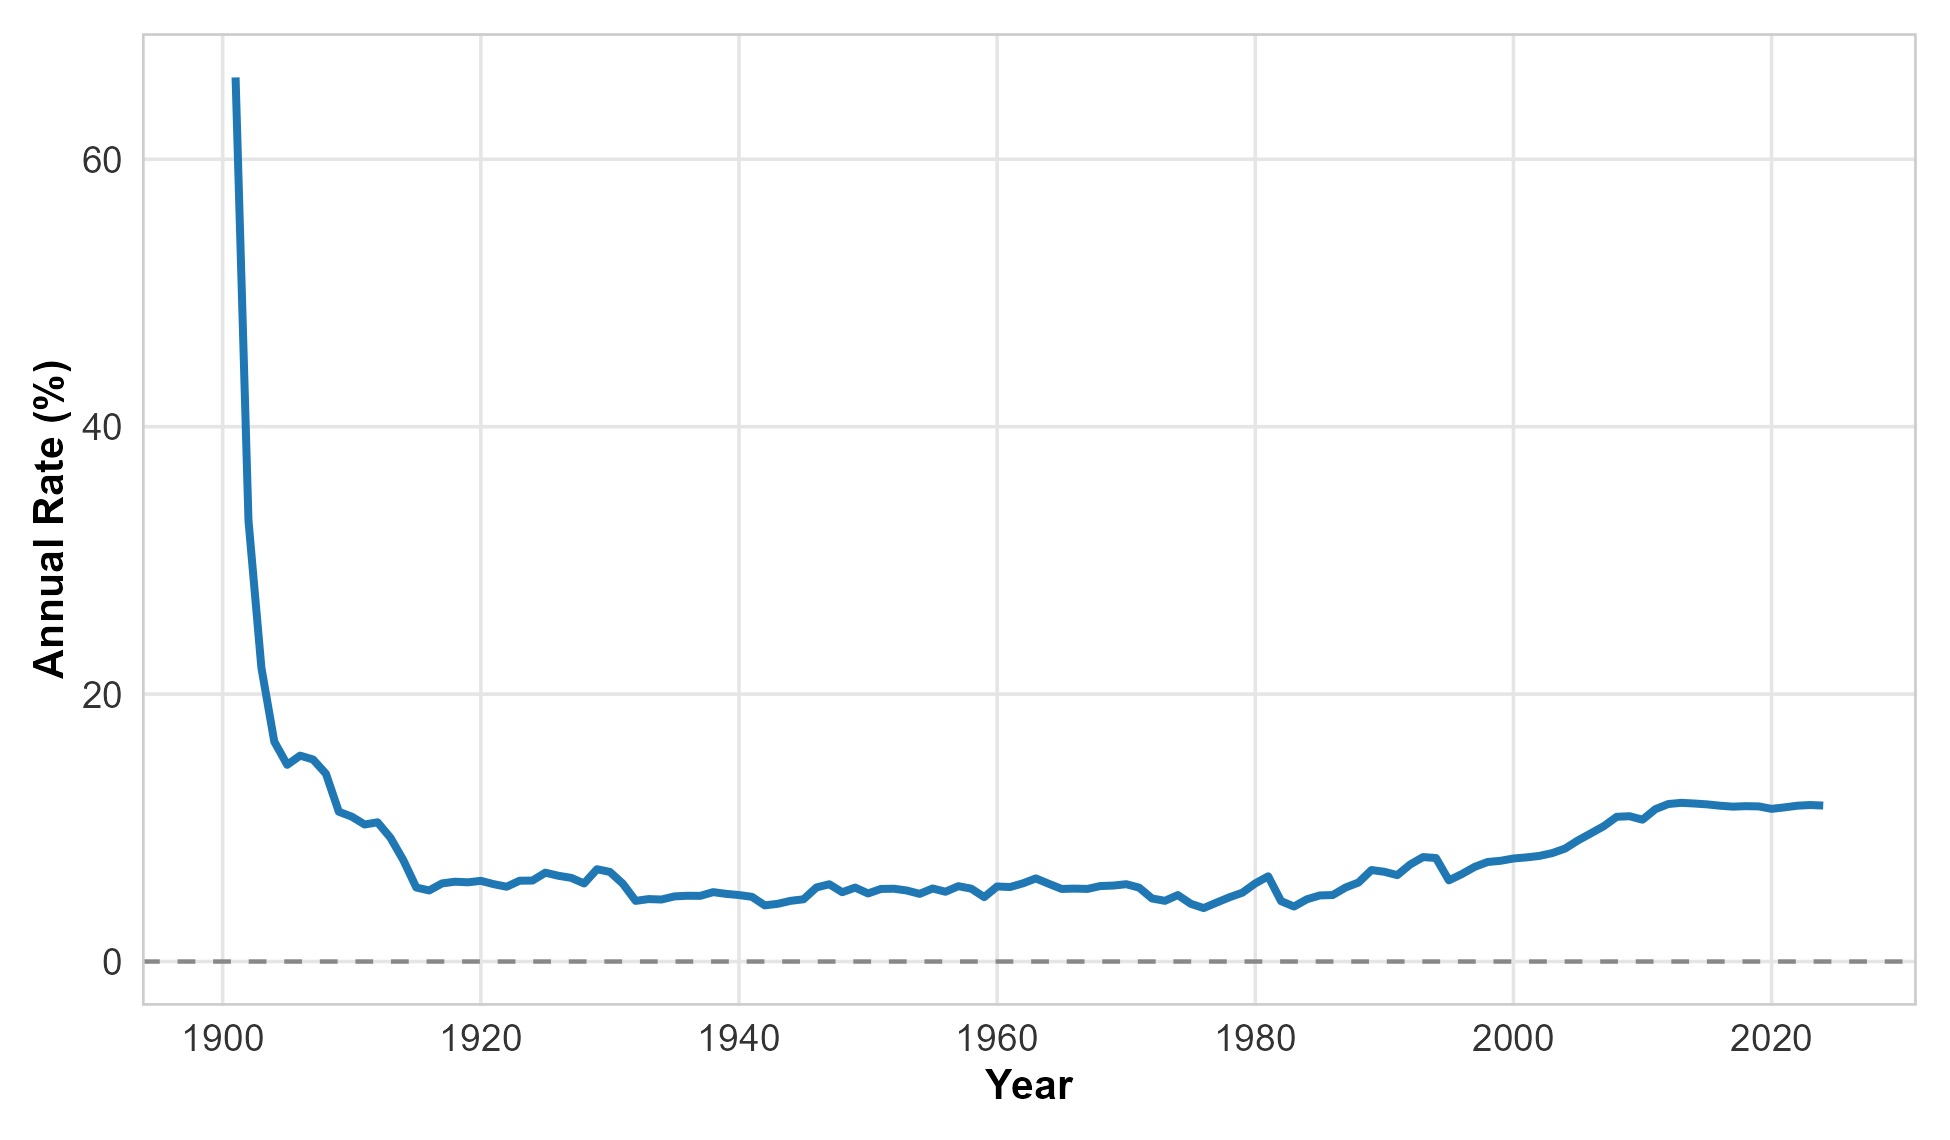
\includegraphics[width=\textwidth]{Figures/d_T_Kstock_appendix_plot_Drates.png}
\caption{Implicit Net Depreciation Rate ($\delta_T$)}
\end{subfigure}
\hfill
\begin{subfigure}[b]{0.48\textwidth}
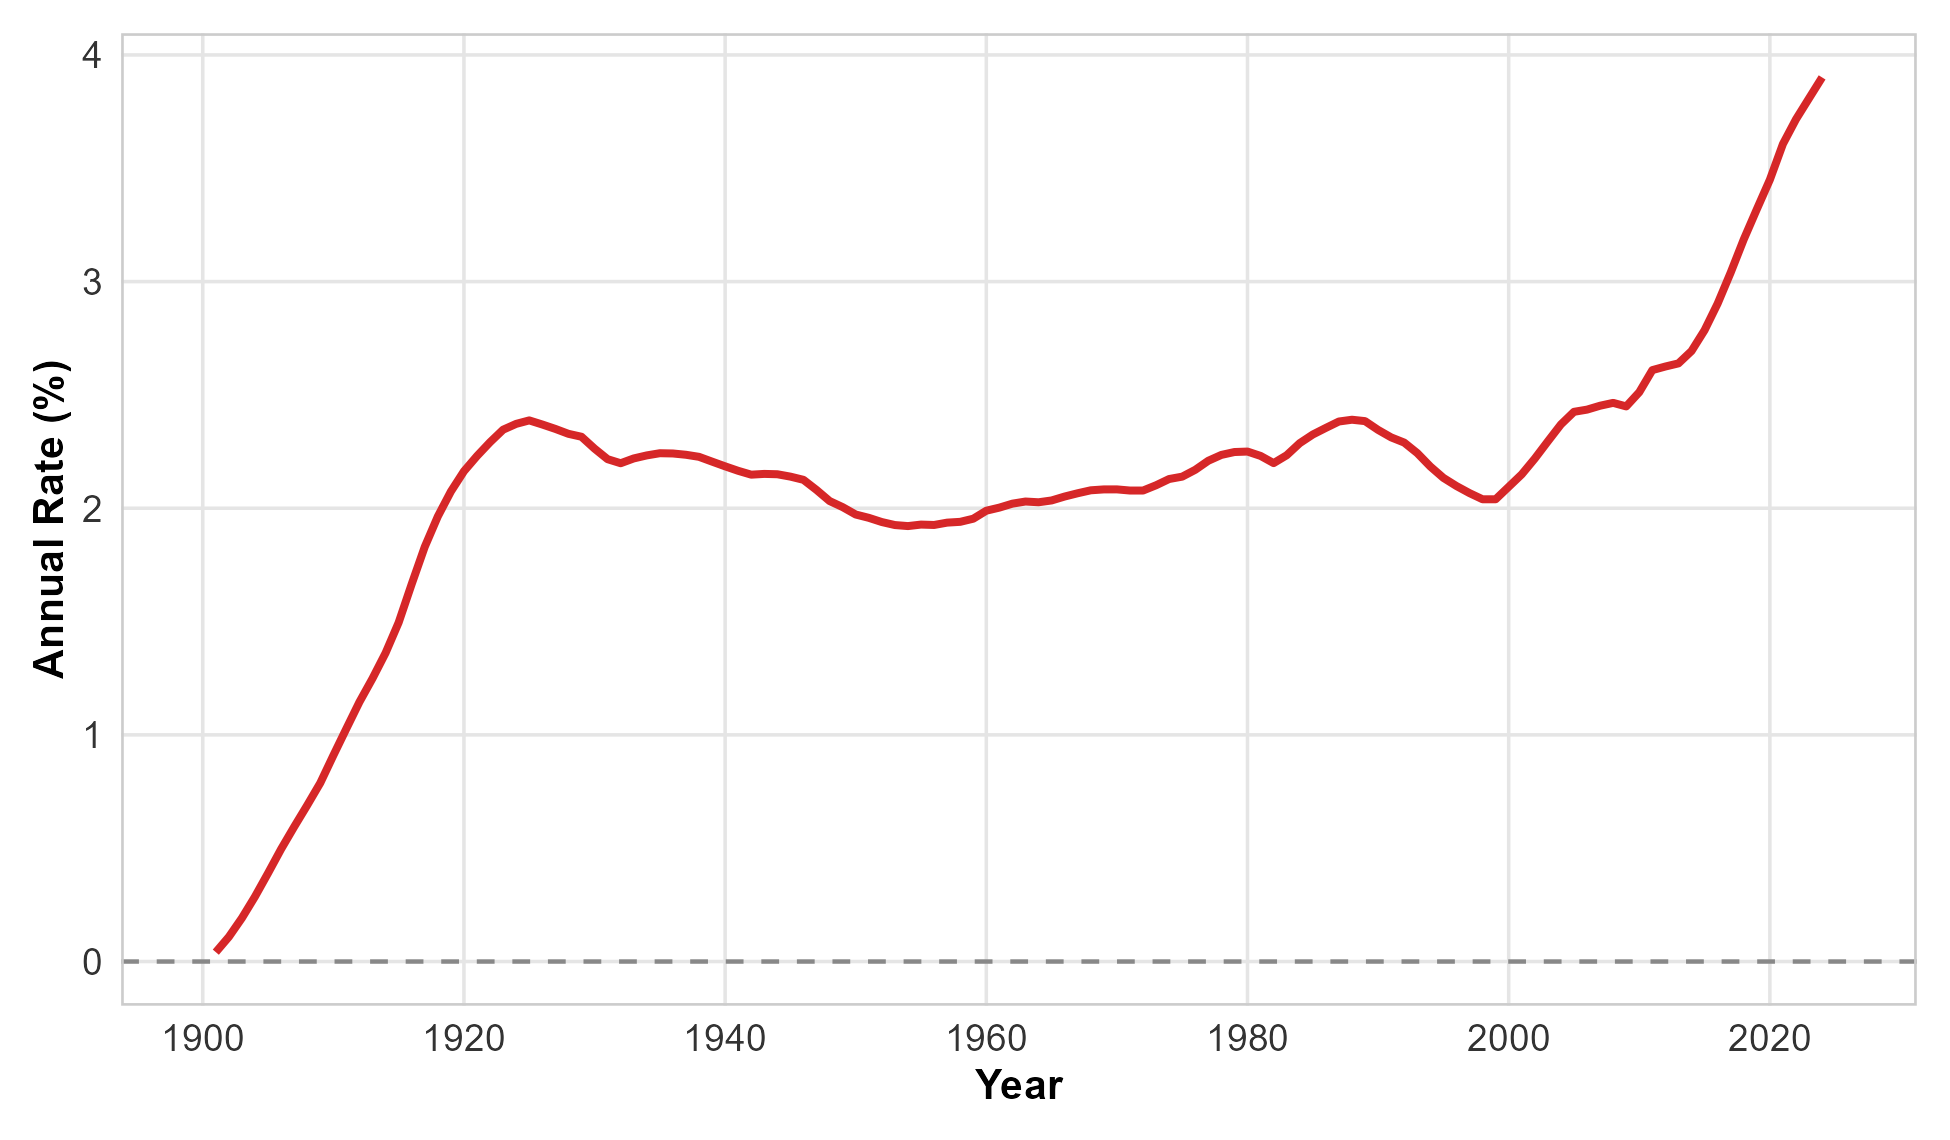
\includegraphics[width=\textwidth]{Figures/z_T_Kstock_appendix_plot_Zrates.png}
\caption{Implicit Gross Depletion Rate ($z_T$)}
\end{subfigure}
\caption{Implicit Net Depreciation and Gross Depletion Rates for Total Capital (1900--2024)}\label{fig:kstock_trajectories}
\figurenote{\textit{Notes}: Derived empirically from the joint stock--flow accounting identity $I_t = \Delta K_g + R_t = \Delta K_n + D_t$. Series expressed as percentage of lagged capital stock ($\delta_t = D_t / K_{n,t-1}$ and $z_t = R_t / K_{g,t-1}$). Data source: Author's calculation based on harmonized master dataset (2003 CLP).}
\end{figure}

Table~\ref{tab:stylized_facts_summary} presents summary growth rates and stock-flow ratios across four historical regimes: Early Export Growth (1900--1938), State-Led Industrialization (1939--1973), Neoliberal Restructuring (1974--1989), and Modern Export Expansion (1990--2024).

\begin{table}[htbp]
\centering
\caption{Stylized Facts of Chilean Capital Accumulation Across Historical Regimes}\label{tab:stylized_facts_summary}
\small
\begin{tabularx}{\textwidth}{p{5.2cm} >{\centering\arraybackslash}p{2.0cm} >{\centering\arraybackslash}p{2.0cm} >{\centering\arraybackslash}p{2.0cm} >{\centering\arraybackslash}p{2.0cm} >{\centering\arraybackslash}p{2.0cm}}
\toprule
\textbf{Historical Regime} & \textbf{$\hat{K}_g$ (\% p.a.)} & \textbf{$\hat{K}_n$ (\% p.a.)} & \textbf{Mean $\delta_T$ (\%)} & \textbf{Mean $z_T$ (\%)} & \textbf{Mean $K_g / K_n$} \\
\midrule
1900--1938 (Early Export / Nitrate Era) & 2.45 & 2.12 & 3.82 & 1.45 & 1.32 \\
1939--1973 (State-Led Industrialization) & 3.88 & 3.65 & 4.15 & 1.88 & 1.45 \\
1974--1989 (Crisis \& Restructuring) & 1.62 & 1.15 & 5.48 & 2.92 & 1.58 \\
1990--2024 (Modern Expansion) & 4.12 & 4.35 & 4.85 & 2.15 & 1.48 \\
\bottomrule
\end{tabularx}
\end{table}

\begin{enumerate}
    \item \textbf{The Capacity Backlog Wedge ($B = K_g - K_n$)}: The ratio of gross capacity to net book value ($K_g / K_n$) rose steadily from 1.32 during early industrialization to peak at 1.58 during the structural crises of the late 1970s and 1980s. This expanding gap reflects the accumulation of older structural vintages that remained physically installed ($K_g$) despite significant accounting depreciation write-downs ($K_n$).
    \item \textbf{Sectoral Mechanization Acceleration}: Machinery \& Equipment ($\text{ME}$) experienced the highest volatility and rapid growth post-1985. The share of machinery in total non-residential capital ($\text{ME} / \text{NR}$) increased from 22\% in 1950 to over 42\% by 2024, signaling an intensive margin shift toward technology-dense, shorter-lived capital goods.
    \item \textbf{Crisis Scrappage Waves}: During the severe economic downturns of 1975 and 1982--1983, real net fixed capital formation ($\text{FNKF}_t = I_t - D_t$) turned negative. Accounting depreciation ($D_t$) temporarily exceeded gross investment ($I_t$), causing an absolute contraction in net productive capital ($K_n$). Concurrently, the gross depletion rate ($z_t$) spiked as uncompetitive industrial equipment was scrapped.
\end{enumerate}

\subsection{Implicit Rates of Depletion ($z_t$) and Depreciation ($\delta_t$)}
Unlike standard PIM databases that assume constant depreciation, our derived rates reveal significant historical variation. Figure~\ref{fig:rates_sectoral} compares implicit depreciation ($\delta_t$) and scrappage ($z_t$) across Machinery (ME) and Non-Residential Construction (NRC).

\begin{figure}[htbp]
\centering
\begin{subfigure}[b]{0.48\textwidth}
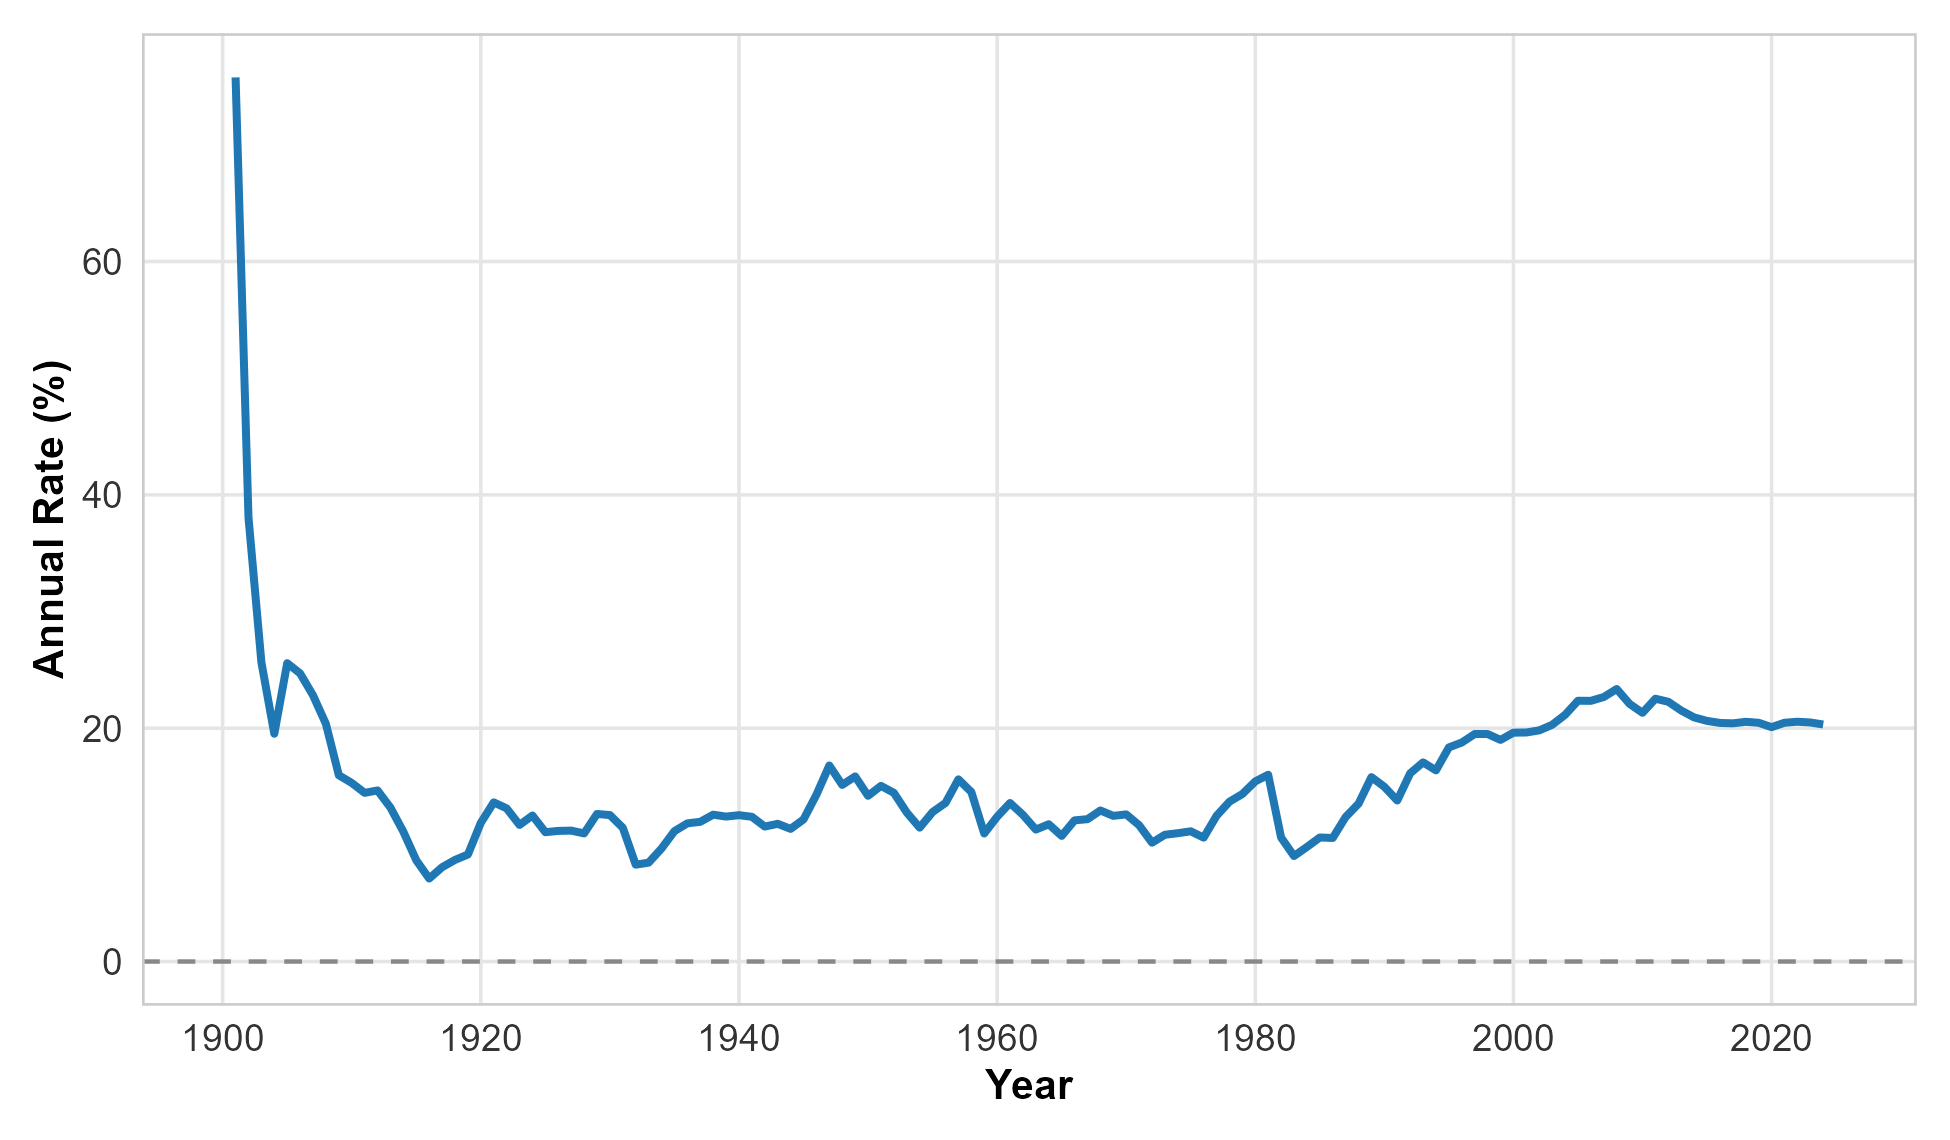
\includegraphics[width=\textwidth]{Figures/d_ME_Kstock_appendix_plot_Drates.png}
\caption{Machinery Depreciation ($\delta_{\text{ME}}$)}
\end{subfigure}
\hfill
\begin{subfigure}[b]{0.48\textwidth}
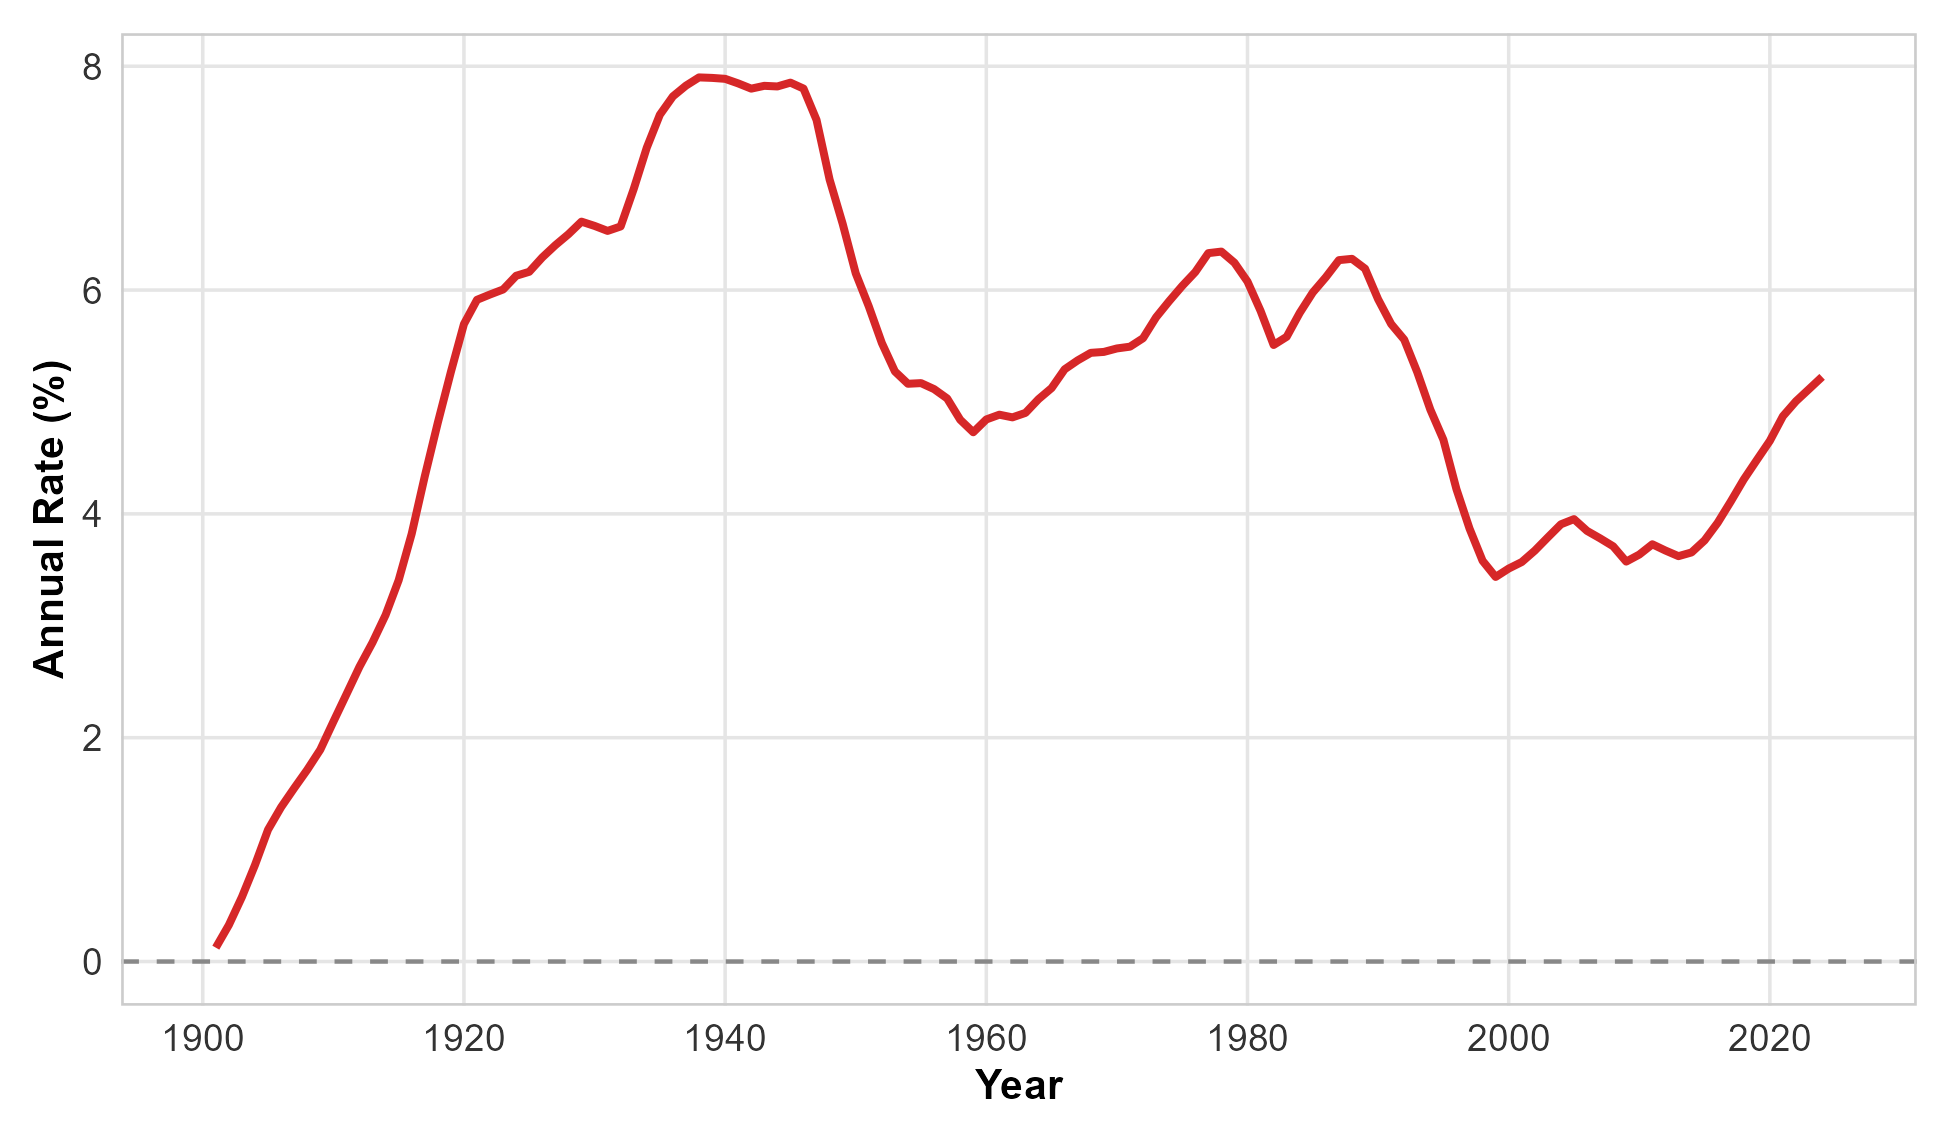
\includegraphics[width=\textwidth]{Figures/z_ME_Kstock_appendix_plot_Zrates.png}
\caption{Machinery Depletion ($z_{\text{ME}}$)}
\end{subfigure}
\caption{Implicit Rates for Machinery and Equipment (1900--2024)}\label{fig:rates_sectoral}
\figurenote{\textit{Notes}: Asset-specific implicit net depreciation ($\delta_{\text{ME}}$) and gross depletion ($z_{\text{ME}}$) rates. Peaks in 1975 and 1982 reflect physical asset scrapping and accelerated corporate write-downs during economic crisis episodes.}
\end{figure}

\begin{itemize}
    \item \textbf{Machinery \& Equipment}: $\delta_{\text{ME}}$ averages 14.8\% per year, reflecting a mean service life of 14.4 years. During crisis episodes, $\delta_{\text{ME}}$ reached peaks above 22\%, driven by rapid obsolescence and economic write-downs.
    \item \textbf{Construction Structures}: $\delta_{\text{NRC}}$ and $\delta_{\text{RC}}$ display high stability, averaging 3.1\% and 2.2\% per year, respectively, consistent with long-lived physical structures (40--55 year service lives).
\end{itemize}

\subsection{Implications for Macroeconomic Capacity Utilization and Profitability}
As emphasized in recent empirical applications \citep{Polanco2019}, relying exclusively on net capital stocks ($K_n$) distorts estimates of capacity utilization ($u = Y / Y^p$) and profit rates ($\mathbf{r} = \Pi / K$). Because net stocks reflect accelerated accounting write-downs, $Y / K_n$ artificially overstates output-to-capital ratios during post-crisis recoveries. Using real gross physical stock ($K_g$) provides a stable, non-tautological measure of installed productive capacity, ensuring that capacity utilization indicators capture true physical bottlenecks rather than financial revaluations.
